\begin{remark}
    The measure of $C_n$ is $(2/3)^n = 0$. From the
    \hyperref[the:continuityOfMeasure]{continuity of measure},
    the measure of the intersection is the limit of measures of individual sets,
    and thus $m(C) = 0$.
\end{remark}

\begin{remark}
    The Cantor set is countable,
    because if we have a sequence of zeros and ones, we can traverse 
    down-left on 0 and down-right on 1. The intersection of the corresponding
    intervals will be a single point of $C$. So, there's a bijection between
    $C$ and $\{0, 1\}^\mathbb{N}$, therefore, $C$ is indeed uncountable. 
\end{remark}

\begin{remark}
    Usually, when we remove the middle intervals on each step,
    we keep the end points.
    If we choose to remove the end points, we essentially remove
    the points that correspond to sequences that end with an infinite
    sequence of 0's or an infinite sequence of 1's. 
    It's clear that not all sequences of 0's and 1's are like that, 
    so there is going to be plenty of points left in the Cantor set, anyway.
\end{remark}

\begin{definition}[The Cantor function]
    The Cantor function $\varphi: [0, 1] \to [0, 1]$ is defined as follows.
    Let's first take the unit interval $[0, 1]$, split it in three,
    and define $\varphi$ to be $\frac{1}{2}$ on $[1/3, 2/3]$. Then let's continue the same
    with $[0, 1/3]$ and $[2/3, 1]$, and so on.

    \begin{figure*}[h]
        \centering
        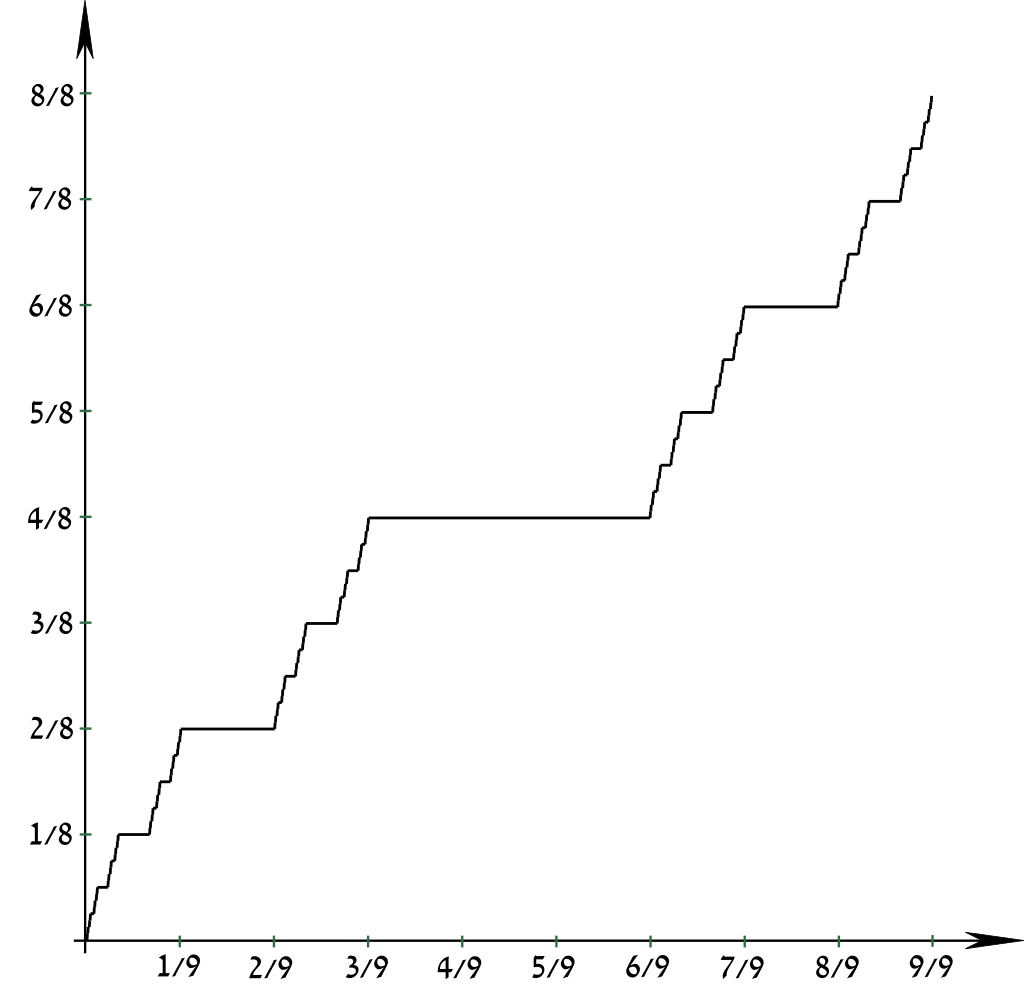
\includegraphics[width=0.4\textwidth]{cantor_function}
    \end{figure*}

    Now we have defined $\varphi$ for all points on the Cantor set. Here's
    how we'll define it on all others:
    \begin{align*}
        &
        O \coloneqq [0, 1] \setminus C
        \\&
        \forall x \in [0, 1] \setminus C:\
        \varphi(x) \coloneqq \sup\{ \varphi(t) \mid t \in C \cap [0, x) \}
    \end{align*}
\end{definition}

\begin{proposition}
    $\varphi$ is increasing, continuous, surjective ($[0,1]$ acts on $[0,1]$),
    $\varphi'$ exists for open set $O$ of measure 1,
    $\varphi'\Bigl|_O \equiv 0$.
\end{proposition}
\begin{proof}
    $\varphi$ is increasing (that's clear), therefore, if $\varphi$ is 
    discontinuous, then it has a jump discontinuity and there will be 
    and interval, say, $I \subset [0,1]$, such that 
    $\varphi([0,1]) \cap I = \emptyset$. But 
    \[ 
        \varphi([0, 1]) \supset \Bigl\{ \frac{m}{2^k} \mathrel{\Big|}
         k \in \mathbb{N}, m \in [0, 2^k]\Bigr\} = K
    \]
    And $K$ is dense in $[0, 1]$, therefore, $K \cap I \ne \emptyset$,
    which is a contradiction.
\end{proof}
\begin{remark}
    The Cantor function is a source of a lot of counterexamples.
    We are going to use it to answer the second question from earlier.
\end{remark}

\begin{definition}
    \[ \psi: [0,1] \to [0,2],\ \psi(x) = \phi(x) + x \]
    $\psi$ is strictly increasing, continuous, surjective.
\end{definition}
\begin{proposition}
    \begin{enumerate}
        \item {
            $\psi$ maps $C$ onto a measurable set of measure 1.
        }
        \item {
            $\psi$ maps some subset of $C$ onto a non-measurable set.
        }
    \end{enumerate}
\end{proposition}
\begin{proof}
    \begin{enumerate}
        \item {
            $m(C) = 0$, thus, $m(O) = m([0, 1] \setminus C) = 1$. We know that
            $\varphi$ is constant on every part of $O$.
            Therefore, $\psi$ looks like $x$ on every part of $O$,
            and there's a countable number of such intervals.
            Therefore, $O$ is mapped to a set of measure 1.
            Thus, $m(\psi(C)) = m(\psi([0, 1])) - m(\psi(O)) = 2 - 1 = 1$.
        }
        \item {
            Since $\psi(C)$ has measure $1 > 0$, by the second homework,
            there exists a non-measurable set $N \subset \psi(C)$. Now
            take $\psi^{-1}(N)$.
        }
    \end{enumerate}
\end{proof}
\begin{corollary}
    \label{cor:measurableNotBorel}
    There is a (measurable) subset of $C$ that is not Borel.
\end{corollary}
\begin{remark}
    Since $m(C) = 0$, the outer measure of each subset of $C$ is also 0,
    thus, every subset of $C$ is measurable. So, the "measurable" part of the 
    corollary is obvious.
\end{remark}
\begin{proposition}
    \label{pro:everyBorIsMeasurable}
    If $f : E \to \mathbb{R}$ is continuous, $E \in \mathcal{M}$, then
    the preimage of every Borel set is measurable.
    \[ \forall B \in \mathcal{B}: f^{-1}(B) = \{ x \in E \mid f(x) \in B \} \in \mathcal{M} \]
\end{proposition}
Let's show how we can prove the corollary if we prove the proposition:
\begin{proof}[Proof of Corollary~\ref{cor:measurableNotBorel}]
    $\psi^{-1}: [0, 2] \to [0, 1]$ is continuous and bijective.
    Let's define $\tilde{C} = \psi^{-1}(N)$. Since $N \subset C$, we have
    $\tilde{C} \subset C$.
    Assume that $\tilde{C}$ is a Borel set, and thus it's measurable.
    Then, by Proposition~\ref{pro:everyBorIsMeasurable},
    its pre-image, $N$, must be measurable as well. But we know it isn't?!
\end{proof}

Let's talk about something more general now, and later return to 
Proposition~\ref{pro:everyBorIsMeasurable}.
\begin{definition}
    $f: X \to Y$ is continuous, if for every open set
    $O \subset Y$, $f^{-1}(O) = \{ x \in X \mid f(x) \in O \}$
    is open in $X$.
\end{definition}
\begin{definition}[Induced topology]
    If $X$ is a topological space and $Y \subset X$,
    the induced topology on $Y$ is defined as follows:
    $O \subset Y$ is open in $Y$ if there exists an open subset
    $\tilde{O} \subset X$ in $X$, such that $O = \tilde{O} \cap Y$.
\end{definition}
